\section{Multi-accelerator Equipped Platform}
Modern compute platforms for scientific computing are evaluated based on their compute power in FLOPS(FLoating Operation Per Second) and memory bandwidth in GB/s (GibaByte Per Second). A single CPU equipped machine, Intel\textsuperscript{\textregistered} Xeon\textsuperscript{\textregistered} Gold 6150 Processor for example, may have 1.3 TFLOP compute power and 120 GB/s memory bandwidth with maximum of 768GB of memory. While a multi-GPU equipped machine, 4 GTX 1080TI for instance, can have aggregately 44 TFLOP compute power and 1936 GB/s memory bandwidth, but only 44 GB of total memory at the same cost. This 33x compute power and 8x memory bandwidth does not come without any cost. Each accelerator can only operate at peak performance for the data allocated at its own memory. Cross GPU data access or inter CPU/GPU data access are significantly slower not only in terms of bandwidth but also in terms of latency, 16GB/s for PCI-E 3.0, 80 GB/s for NVLink 1.0 and 150 GB/s for NVLink 2.0. A heterogeneous platform often refers to those type of machines that not all resources can be accessed at the same cost across the platform. For instance, a GPU(GTX 1080TI as an example) may be able to access data allocated on its own memory at 484GB/s, but for accessing data allocated on CPU, it would require communication across PCI-E at maximum speed 16GB/s with couple of microsecond latency. 

\begin{figure}[t!]
\includegraphics[height=.4\textwidth]{images/DD/Teaser_Part1.png}
\includegraphics[height=.4\textwidth]{images/DD/Teaser_Part2_5x4.png}
%\includegraphics[width=.33\textwidth]{images/teaser_dragon_splash.png}
%\includegraphics[width=.33\textwidth]{images/teaser_snake_channel.png}
%\includegraphics[width=.33\textwidth]{images/teaser_flasks.png}
\caption{Left: Smoke injected into a model of the bronchi. Color illustrates vorticity magnitude. Simulation contains 1.8 billion active cells, sparsely
  occupying a $8192^2\!\times\!4096$ background grid. Right: Smoke injected from the bottom of a cylinder, and forced through a metal gasket (rendered semi-transparent) with a
  twisted bundle of cylindrical holes. Total of 1.2 billion active cells, in a $1024^2\!\times\!2048$ background grid.}
\label{fig:DD-teaser}
\end{figure}

When designing algorithms for a heterogeneous platform, the locality of data need always be kept in mind for best utilization of the computing resources, otherwise, in the most unfortunate case, only a memory speed of 16GB/s maybe utilized, instead of the ideal 1936 GB/s. In such a case, the single CPU platform with 140 GB/s memory bandwidth may better perform this multi-GPU equipped machine. It should be noted that this non-uniformity of bandwidth is not an aberration of hardware design that is likely going away; in fact it is consistent with the fact that memory
hierarchies, and physical proximity of memory to computational units, have long given rise to differentiation in latency and bandwidth between different parts of the computational
platform.

Unfortunately, some of the best performing solvers (in terms of convergence efficiency) such as multigrid are the cases of the worst scenarios. The building blocks of a multigrid
solver, namely the smoothing routine and transfer operators, require global synchronization after their execution while carrying out only a very modest amount of useful computation
in between synchronization points. In particular, a Jacobi or Gauss-Seidel style smoother requires no more than two passes over the data in memory, which completes in a very small
fraction of the cost incurred for transferring the data to the GPU card, or out of it upon completion. Of course, one could take the opportunity to carry out several smoothing
iterations per offload operation; however, without synchronization at partition boundaries this extra effort will hardly translate to worthwhile gains in convergence. As a result,
the benefit of the GPU offload is negated, and such large problems are better off being solved homogeneously on the CPU. Although there might be room for implementation refinements
and adaptation of multigrid paradigms to curb this overhead, we are not aware of prior work that has demonstrated viability of a GPU-offload paradigm for multigrid solvers, when
the problem size exceeds the memory capacity of the GPU card(s), compare to a well-optimized CPU implementation. Our proposed approach directly addresses this challenge: instead of
executing just a few iterations of a smoother routine, we run an entire solver routine on the GPU for each independent subdomain we offload to it. In our case, that extra effort
does translate to accelerated convergence, and the GPU computation is long enough to absorb the transfer cost.
\section{Domain Decomposition as Divide-and-conquer}
In this chapter, a Schur Complement domain decomposition method is presented, the objective is to demonstrate an effective, and hopefully inspiring adaptation to fluids simulation of a class of numerical techniques that has received much more exposure in scientific computing than graphics research. We note, however, that Schur Complement methods provide a general framework, and not just a singular algorithm; in fact, similar to multigrid methods, careful variations from the general algebraic theme make all the difference between a given scheme being highly effective or underwhelming for a specific application. In this vein, we consciously restricted the scope of our investigation to just uniform discretizations of fluids, specifically targeted the Poisson equation (although our formulations should readily extend to elasticity, or other elliptic problems), and did not emphasize the implications of heterogeneous computing to other parts of the fluid simulation pipeline.

The classical divide-and-conquer paradigm encountered in combinatorial algorithms often presumes building blocks that accurately solve subsets of the overall problem. In our numerical context, one of the key opportunities we will exploit is the option to design what is not an exact solver, but an excellent approximation of one, and subsequently use it as a preconditioner. In this context, we will adopt a slightly different standard which we will design our ``inaccurate'' divide-and-conquer scheme to satisfy. Our building block will be an inexact solver for the Poisson equation on independent partitions of our domain, which is however of good enough quality to be used as an excellent Conjugate Gradients preconditioner (i.e. it would lead to convergence in a small number of iterations, that does not significantly increase as the subdomain size grows larger). Subsequently, our objective would be to combine such ``nearly accurate'' building blocks into a global approximate solver that meets the same benchmark, i.e. it can be used as a highly effective preconditioner that allows CG to converge in a comparably small number of iterations as its individual constituents. We note that,short of this standard, using divide-and-conquer tricks can be a slippery slope and result is significantly degraded performance.

\section{The classic Schur complement method}
\label{sec:dd-fundamentals}

We introduce the basic principles of the Schur complement method [\cite{quarteroni:1999:domain}] by explaining how an aggregate solver for the pressure Poisson
equation can be assembled using as subroutines two independent solvers for two non-overlapping partitions of the entire computational domain.
After covering the basic theory we will detail how this construction extends to multiple partitions, and derive a preconditioner based on this concept in later sections.

\subsection{The two-subdomain case}

\begin{wrapfigure}{r}{.25\columnwidth}
\mbox{
  \begin{overpic}[width=.3\columnwidth]{images/DD/two_subdomains.pdf}
    \put(15,15){$\Omega_1$}
    \put(60,50){$\Omega_2$}
    \put(82,8){$\Gamma$}
  \end{overpic}}
\end{wrapfigure}
Consider a domain $\Omega$ that has been partitioned into two subdomains
$\Omega_1$ and $\Omega_2$ through an interface region $\Gamma$. Let us assume we have a
finite-difference discretization of the pressure Poisson equation on $\Omega$,
and that the interfacial region $\Gamma$ is thick enough to shield any stencil in $\Omega_1$ from including a point in $\Omega_2$ (and vice-versa).  In
practice, when using the standard $7$-point stencil in a Cartesian discretization, the interface layer $\Gamma$ can simply be one-node thick as long as it cleanly
decouples $\Omega$ into two distinct subdomains (although $\Gamma$ could also be made wider, if desired). For simplicity of notation we will write the Poisson
equation as $Ax=b$, with the understanding that the vector $x$ contains the unknown pressure values and $b$ contains the respective divergence values of the velocity
field. We then reorder degrees of freedom as:
% to group together degrees of freedom in $\Omega_1$, $\Omega_2$ and $\Gamma$ as follows:
%When solving the Poisson equation $Ax=b$ on $\Omega$, if the degrees of freedom have been reordered such that
\begin{eqnarray}
\label{eqn:dof}
x=
\begin{bmatrix}
x_1 \\
x_2 \\
x_\Gamma
\end{bmatrix}
,\enspace\enspace\enspace\enspace
b=
\begin{bmatrix}
b_1 \\
b_2 \\
b_\Gamma
\end{bmatrix}
\end{eqnarray}
where $x_i,b_i$ correspond to values in $\Omega_i$, for $i\in\{1,2\}$ (and similarly $x_\Gamma,b_\Gamma$ correspond to degrees of freedom in $\Gamma$). Under this
reordering, the matrix $A$ assumes the following block form:
\begin{eqnarray}
\label{eqn:block-sparsity-A}
A=
\begin{bmatrix}
A_{11} & & A_{1\Gamma} \\
& A_{22} & A_{2\Gamma} \\
A_{\Gamma 1} & A_{\Gamma 2} & A_{\Gamma\Gamma}
\end{bmatrix}
\end{eqnarray}
Note that due to symmetry of $A$, we have $\varB{A}_{\Gamma 1}^T\!\!=\!\!\varB{A}_{1\Gamma}$ and $\varB{A}_{\Gamma 2}^T\!\!=\!\!\varB{A}_{2\Gamma}$ for the off-diagonal blocks.
Using this block form of $A$ it is possible to write the following factorization of the \emph{inverse} matrix $A^{-1}$:
\begin{eqnarray*}
\label{eqn:block-factorization-A}
\varB{A}^\varA{-1}\!=\!\!
\begin{bmatrix}
I & & \varB{-A}_{11}^\varA{-1}A_{1\Gamma} \\
& I & \varB{-A}_{22}^\varA{-1}A_{2\Gamma} \\
\ \ \ \tikzmark{c1} & & \ \ \ \ I\ \ \ \ \tikzmark{c2}
\end{bmatrix}
\hspace{-.2cm}
\begin{bmatrix}
\!A_{11}^\varA{-1}\!\!\! & & \\
& \!\!\!\!A_{22}^\varA{-1}\!\! & \\
\!\tikzmark{d1} & & \!\!\!\Sigma^\varA{-1}\!\tikzmark{d2}
\end{bmatrix}
\hspace{-.2cm}
\begin{bmatrix}
I & & \\
& I & \\
\tikzmark{ct1}\varB{-A}_{\Gamma 1}A_{11}^\varA{-1} & \varB{-A}_{\Gamma 2}A_{22}^\varA{-1} & I\tikzmark{ct2}
\end{bmatrix}
\begin{tikzpicture}[overlay, remember picture,decoration={brace,amplitude=5pt}]
\draw[decorate,thick] (c2.south) -- (c1.south)
      node [midway,below=5pt] {$U$};
\draw[decorate,thick] (d2.south) -- (d1.south)
      node [midway,below=5pt] {$D$};
\draw[decorate,thick] (ct2.south) -- (ct1.south)
      node [midway,below=5pt] {$U^T$};
\end{tikzpicture}
\end{eqnarray*}

where
$$\Sigma=A_{\Gamma\Gamma}-A_{\Gamma 1}A_{11}^\varA{-1}A_{1\Gamma}-A_{\Gamma 2}A_{22}^\varA{-1}A_{2\Gamma}$$
is the \emph{Schur complement} of the block $A_{\Gamma\Gamma}$ in equation (\ref{eqn:block-sparsity-A}).
The validity of this factorization can be verified via a direct substitution into the identity $A\!\cdot\!A^{-1}\!=\!I$.
 Finally, since $A$ (and its inverse) is a symmetric positive definite(SPD) matrix, this factorization
implies that the Schur complement is also symmetric and positive definite (the matrix $D$ is equal to the symmetric conjugation of the symmetric positive definite
matrix $A^{-1}$ with the matrix $U^{-1}$; hence its diagonal sub-block $\Sigma^{-1}$ is symmetric definite, too).

\begin{figure*}[h]
\tiny
\begin{align}
\label{eqn:factorization-k-subdomains-exact}
\hspace{-3cm} A^\varA{-1} &=
\begin{bmatrix}
I & & & \varB{-A}_{11}^\varA{-1}A_{1\Gamma} \\
& \ddots & & \vdots \\
& & I & \varB{-A}_{kk}^\varA{-1}A_{k\Gamma} \\
& & & I
\end{bmatrix}
\begin{bmatrix}
A_{11}^\varA{-1} & & & \\
& \ddots & & \\
& & A_{kk}^\varA{-1} & \\
& & & \Sigma^\varA{-1}
\end{bmatrix}
\begin{bmatrix}
I & & & \\
& \ddots & & \\
& & I & \\
\varB{-A}_{\Gamma 1}A_{11}^\varA{-1} & \ldots & \varB{-A}_{\Gamma k}A_{kk}^\varA{-1} & I
\end{bmatrix} \\
\label{eqn:factorization-k-subdomains-five}
&=
\begin{bmatrix}
A_{11}^\varA{-1} & & & \\
& \ddots & & \\
& & A_{kk}^\varA{-1} & \\
& & & I
\end{bmatrix}
\begin{bmatrix}
I & & & \varB{-A}_{1\Gamma} \\
& \ddots & & \vdots \\
& & I & \varB{-A}_{k\Gamma} \\
& & & I
\end{bmatrix}
\begin{bmatrix}
A_{11} & & & \\
& \ddots & & \\
& & A_{kk} & \\
& & & \Sigma^\varA{-1}
\end{bmatrix}
\begin{bmatrix}
I & & & \\
& \ddots & & \\
& & I & \\
\varB{-A}_{\Gamma 1} & \ldots & \varB{-A}_{\Gamma k} & I
\end{bmatrix}
\hspace{-.2cm}
\begin{bmatrix}
A_{11}^\varA{-1} & & & \\
& \ddots & & \\
& & A_{kk}^\varA{-1} & \\
& & & I
\end{bmatrix} \\
\label{eqn:factorization-k-subdomains-approx-five}
&\approx
\begin{bmatrix}
\textcolor{red}{A_{11}^\dagger} & & & \\
& \ddots & & \\
& & \textcolor{red}{A_{kk}^\dagger} & \\
& & & I
\end{bmatrix}
\hspace{-.2cm}
\begin{bmatrix}
I & & & \varB{-A}_{1\Gamma} \\
& \ddots & & \vdots \\
& & I & \varB{-A}_{k\Gamma} \\
& & & I
\end{bmatrix}
\hspace{-.2cm}
\begin{bmatrix}
I & & & \\
& \ddots & & \\
& & I & \\
& & & \textcolor{red}{\Sigma^\dagger}
\end{bmatrix}
\hspace{-.15cm}
\left\{
I+
\begin{bmatrix}
& & & \\
& & & \\
& & & \\
\varB{-A}_{\Gamma 1} & \ldots & \varB{-A}_{\Gamma k} & I
\end{bmatrix}
\hspace{-.2cm}
\begin{bmatrix}
\textcolor{red}{A_{11}^\dagger} & & & \\
& \ddots & & \\
& & \textcolor{red}{A_{kk}^\dagger} & \\
& & & I
\end{bmatrix}
\right\}
\end{align}
\normalsize
\end{figure*}

\subsection{The multiple subdomain solver}
\begin{figure*}[t!]
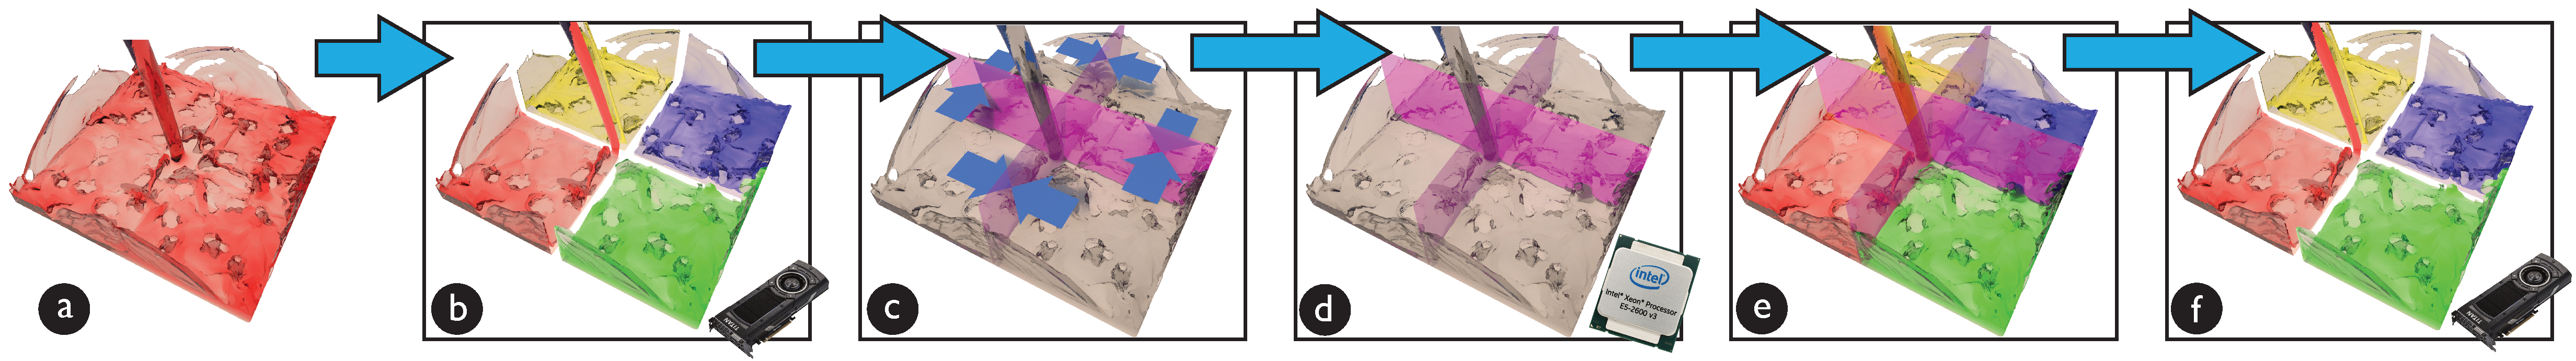
\includegraphics[width=\textwidth]{images/DD/SolverStages.pdf}
\caption{Illustration of the core concept of our method: (b) We split the computational grid into subdomains, and independently solve them on the GPU(s), using
  zero Dirichlet conditions on subdomain boundaries. (c) Fluxes of the subdomain solutions are computed and sent to 
  the CPU. (d) A specially formulated system is solved on the interface, using the CPU. This produces the exact value of the interface variables. (e) Those
  values are sent to the subdomains, and set as Dirichlet conditions. (e) A final subdomain solve on the GPU yields the global solution.}
\label{fig:pipeline}
\end{figure*}
This formulation extends naturally to an arbitrary number of $k$ subdomain partitions $\Omega_1,\ldots,\Omega_k$ separated by an interface set $\Gamma$ (figure
\ref{fig:pipeline} depicts such a partitioning into four subdomains, with the interface $\Gamma$ highlighted as the magenta-colored separator surface). The
corresponding factorization of $A^{-1}$ in this case is given in equation (\ref{eqn:factorization-k-subdomains-exact}). In order to translate this algebraic expression
into a solver algorithm, we first re-factor this into the five-matrix product of equation (\ref{eqn:factorization-k-subdomains-five}), which has every subdomain
inverse $A_{ii}^\varA{-1}$ appear only twice (as opposed to three inversions per subdomain, in equation \ref{eqn:factorization-k-subdomains-exact}). The last
algebraic manipulation, as given in equation (\ref{eqn:factorization-k-subdomains-approx-five}) further avoids the appearance of the subdomain Laplacian
$A_{ii}$, requiring only the inverses of such matrices. In this expression we have also substituted the symbol ${\color{red}M^\dagger}\approx M^{-1}$ for
\emph{approximate} inverses of $A_{ii}$ and $\Sigma$. If the \emph{exact} inverse of these matrices was used, equation (\ref{eqn:factorization-k-subdomains-approx-five})
becomes identically equal to the five-factor expression of equation (\ref{eqn:factorization-k-subdomains-five}). We will later engage in such approximations; for now, we
may assume that all these inverses are exact.  


%  The reader is
% welcome to verify the accuracy of this factorization via simple algebraic
% substitution. Since the matrix $A$ is symmetric and positive-definite (and hence, $A^\varA{-1}$),
% it follows from the factorization that the matrix $D$ is symmetric and positive-definite. 
% The symmetry and positive-definiteness of the matrix $\Sigma$ now follows from
% the fact that both the matrices $A_{11}$ and $A_{22}$ are symmetric and positive-definite.
% Equivalently, $A^\varA{-1}$ can also be factorized as $A=C'D'C'^T$, where

% \begin{eqnarray*}
% \label{eqn:equivalent-block-factorization-A}
% C'=
% \begin{bmatrix}
% A_{11}^\varA{-1} & & \\
% & A_{22}^\varA{-1} & \\
% & & I
% \end{bmatrix}
% \hspace{-.2cm}
% \begin{bmatrix}
% I & & \varB{-A}_{\Gamma 1} \\
% & I & \varB{-A}_{\Gamma 2} \\
% & & I
% \end{bmatrix}, \enspace\enspace
% D'=
% \begin{bmatrix}
% I & & \\
% & I & \\
% & & \Sigma^\varA{-1}
% \end{bmatrix}
% \end{eqnarray*}
% This factorization only requires computation of
% the inverses $A_{11}^\varA{-1}$ and $A_{22}^\varA{-1}$ for the individual subdomains.
% Multiplying the vector $b$ from equation (\ref{eqn:dof}) with
% this factorization
% from right to left yields the following algorithm for solving the original system
% $Ax=b$:

The Schur complement method effectively solves the equation $Ax=b$ by multiplying the right hand side $b$ with the factorized equivalent of $A^{-1}$ from equation 
(\ref{eqn:factorization-k-subdomains-approx-five}). The key observation is that we can apply this multiplication indirectly, without explicitly constructing the
matrix in this factorization. We do this as follows:
\vspace*{-.15in}
\begin{enumerate}
\item
Solve $k$ subproblems: $A_{11}\hat x_1=b_1$, \ldots,  $A_{kk}\hat x_k=b_k$.
\vspace*{-.05in}
\item
Solve $\Sigma x_\Gamma=b_\Gamma-A_{\Gamma 1}\hat x_1-A_{\Gamma 2}\hat x_2 - \ldots -A_{\Gamma k}\hat x_k $.
\vspace*{-.05in}
\item
Solve the $k$ new subproblems\\ $A_{11}\delta x_1=-A_{1\Gamma}x_\Gamma$, \ldots, $A_{kk}\delta x_k=-A_{k\Gamma}x_\Gamma$.
\vspace*{-.05in}
\item
Update $x_1\leftarrow \hat x_1+\delta x_1$, \ldots, $x_k\leftarrow \hat x_k+\delta x_k$.
\end{enumerate}
Observe that steps ($1$) and ($3$) require the solution of fully decoupled systems for each subdomain $\Omega_i$, and this can easily be performed in
parallel without any need for communication or synchronization.
Step ($2$) requires the solution of a symmetric and positive definite system (with the Schur complement $\Sigma$ as the
coefficient matrix). Traditionally, solvers based on this method attempt to solve this interface system using a preconditioned Krylov
subspace method such as Conjugate Gradients. We will deviate from
this practice, and use equation (\ref{eqn:factorization-k-subdomains-approx-five}) instead, to design a preconditioner for the \emph{global} (coupled) system.

 It is important to examine the algebraic structure of $\Sigma$, and assess the performance implications of attempting to solve the system in step (2) directly.
 For a volumetric
domain $\Omega$ with $N$ total degrees of freedom, the dimensionality of $\Gamma$ would be $O(\sqrt{N})$ in 2D, and $O(N^{2/3})$ in 3D. Note, however, that in contrast to the
sparse Laplace matrix $A$, the Schur complement is a dense matrix, thus having $O(N^{4/3})$ entries and requiring at least as much computation to solve. Asymptotically, this would
make step (2) above by far the bottleneck of the solver, if $\Sigma$ was to be explicitly constructed. Furthermore, the construction of the matrix alone would likely require even
more computation, as it would need to account for computing the subdomain inverses $A_{ii}^\varA{-1}$. Using Conjugate Gradients as the solver in step (2) opens up an interesting
possibility: the CG algorithm does not need an explicitly constructed matrix $\Sigma$, as long as we have a way to compute matrix-vector products $\Sigma x_\Gamma$. In turn, this
would require computing products of the form $A_{\Gamma i}A_{ii}^\varA{-1}A_{i\Gamma}x_\Gamma$ as efficiently as possible. Although the factors $A_{\Gamma i}$, $A_{i\Gamma}$ are
sparse enough to allow efficient multiplication, multiplying with $A_{ii}^\varA{-1}$ (i.e. solving a subdomain Poisson problem) requires at least linear cost relative to the size
of the subdomain (assuming a linear-complexity solver, like an extremely well built multigrid scheme, iterated to full convergence). There would be opportunity for parallelization
across subdomains, but we would be still confronted with a linear complexity cost for \emph{each} CG iteration, and we would have to rely on constructing an extremely efficient
preconditioner to ensure that only a small finite number of iterations would suffice, independent of resolution. Nevertheless, this is the
  path followed by many derivative techniques
of the Schur complement method (often referred to as \emph{iterative substructuring}; an excellent synopsis of such options is given in the classic book by \cite{quarteroni:1999:domain}).

